\documentclass[12pt]{article}
\usepackage{amsmath,amssymb}
\setlength{\oddsidemargin}{0in}
\setlength{\evensidemargin}{0in}
\setlength{\textheight}{9in}
\setlength{\textwidth}{6.5in}
\setlength{\topmargin}{-0.5in}
\usepackage{enumitem}
\usepackage[table]{xcolor}
\usepackage{graphicx}
\usepackage{listings}
\usepackage{float}
\usepackage{caption}
\usepackage{subcaption}
\newcommand{\Adv}{{\mathbf{Adv}}}       
\newcommand{\prp}{{\mathrm{prp}}}             
\newcommand{\calK}{{\cal K}}
\newcommand{\outputs}{{\Rightarrow}}                



% Use \textbf{Solution:}\\ to begin your solution.

%%%%%%%%%%%%%%%%%%%%%%%%%%%%%%%%%%%%%%%%%%%%%%%%%%%%%%%%%%%%%%%%%%%%%%%%%%%
\title{\bf Math 151A: Problem Set 3}
\date{5/1/2023}
\author{\bf Owen Jones}

\begin{document}
\maketitle

%Add \newpage  between problems if you are using this to LaTex your solutions
\vspace{1em}

%%%%%%%%%%%%%%%%%%%%%%%%%%%%%%%%%%%%%%%%%%%%%%%%%%%%%%%%
\begin{enumerate}[label=\bfseries Problem \arabic*:]

 %%%%%%%%%%%%%%%%%%%%%%%%%%%%%%
 \item \textbf{(C) Newton's Method}\\
  Use Newton's method to find solutions accurate to within $10^{-5}$ for the problem:
$$e^x +2^{-x} +2 \cos{x}-6=0 \ \text{for} \  1\leq x \leq 2.$$
 Repeat using the Secant method. Report the number of iterations needed to reach your computed solutions. 
 
 \textit{For this problem:  The true root is $p=1.82938360193385$, you can use the stopping criterion: $|p_n-p|\leq 10^{-5}$. }

\vspace{1em}
\textbf{Solution:}\par 
$f\in C^2[1,2]$, $p\in(1,2)$, $f(p)=0$ $f'(p)\neq0$, so there exists a sequence $(p_n)^{\infty}_{n=1}$ that converges to $p$ for any initial $p_0$ within some $\delta$ of $p$. Let $p_0=1$, (and $p_1=1.5$ for secant method). \textit{Number of iterations and approximations of p for both methods shown in the command window accompanying code.} \par 
\begin{figure}[H]
  \begin{subfigure}[t!]{.5\textwidth}
  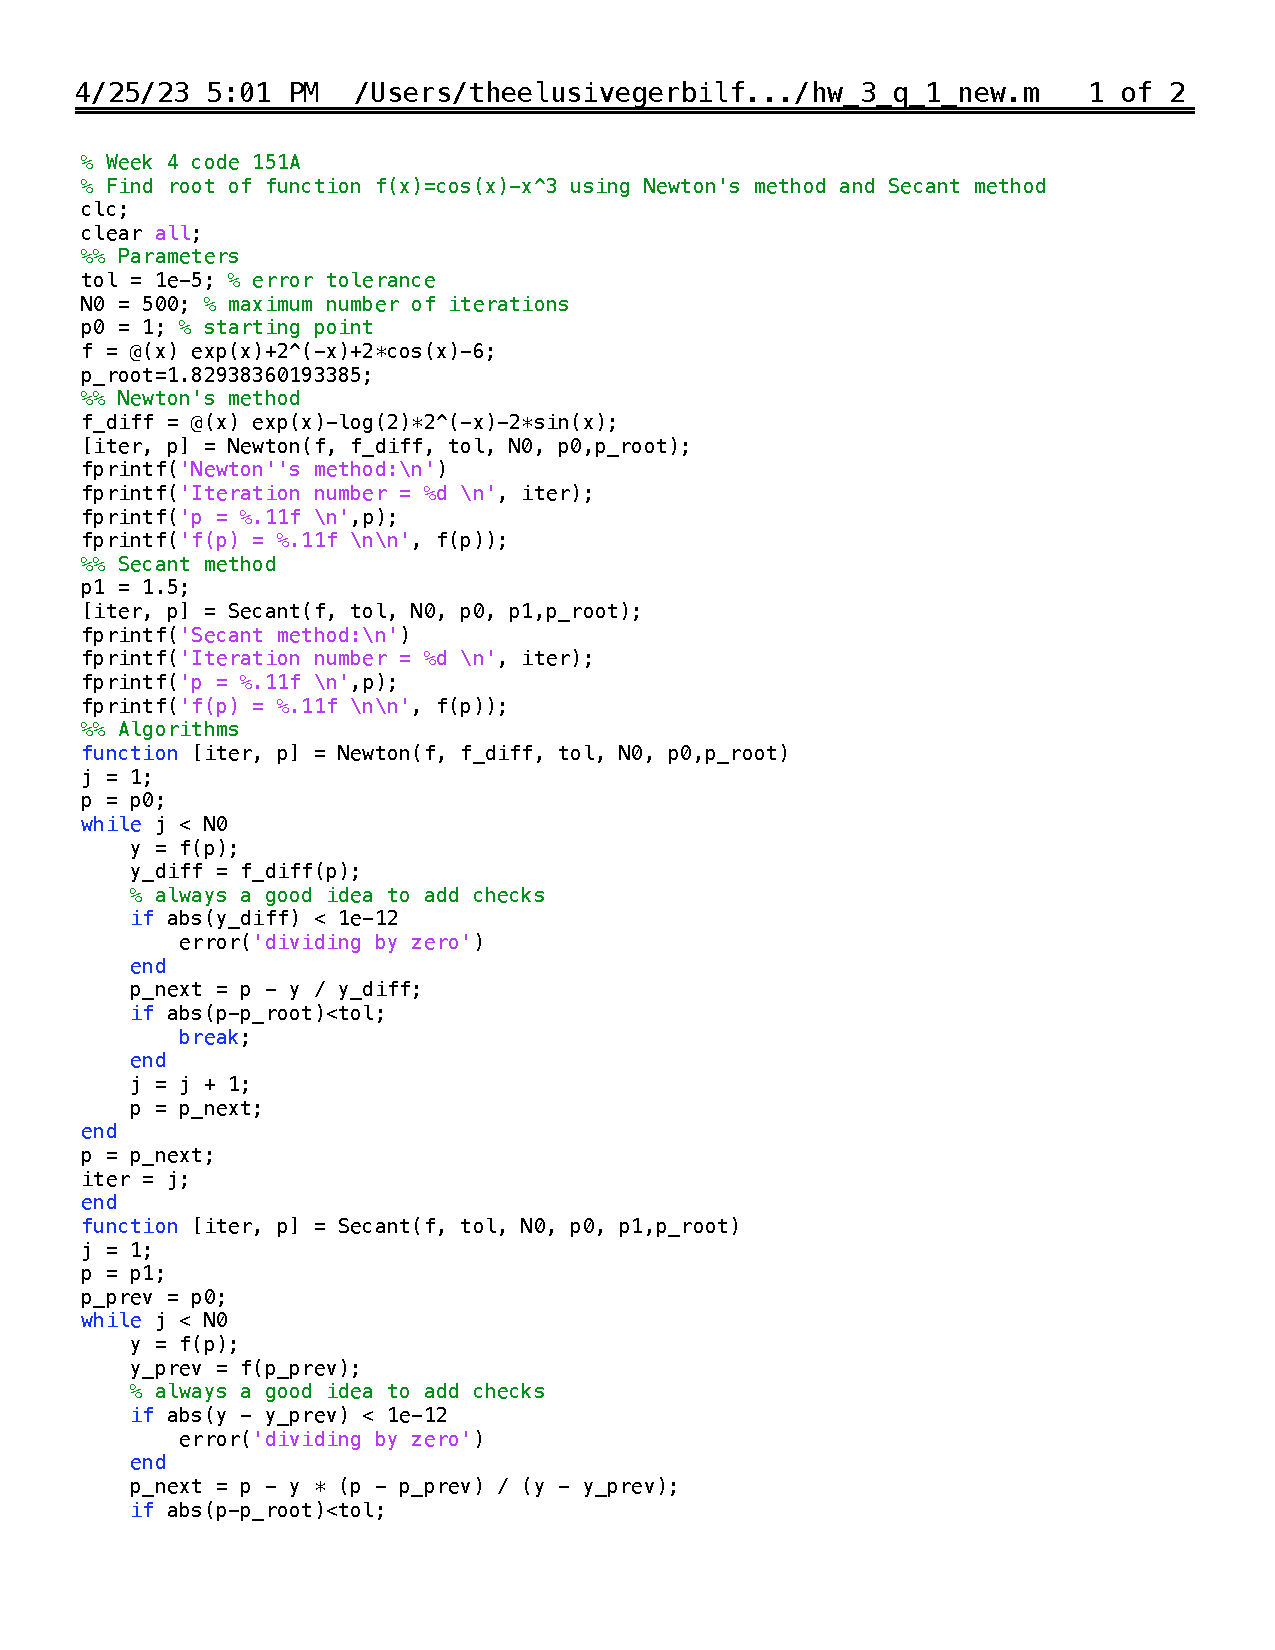
\includegraphics[clip, trim=0 2.1cm 0 0, page=1, width=\linewidth]{Newton_hw_3_q_1_new.pdf} 
  \includegraphics[clip, trim=0 20cm 0 2.6cm, page=2, width=\linewidth]{Newton_hw_3_q_1_new.pdf}
  \end{subfigure}%
  \begin{subfigure}[t!]{.5\textwidth}
  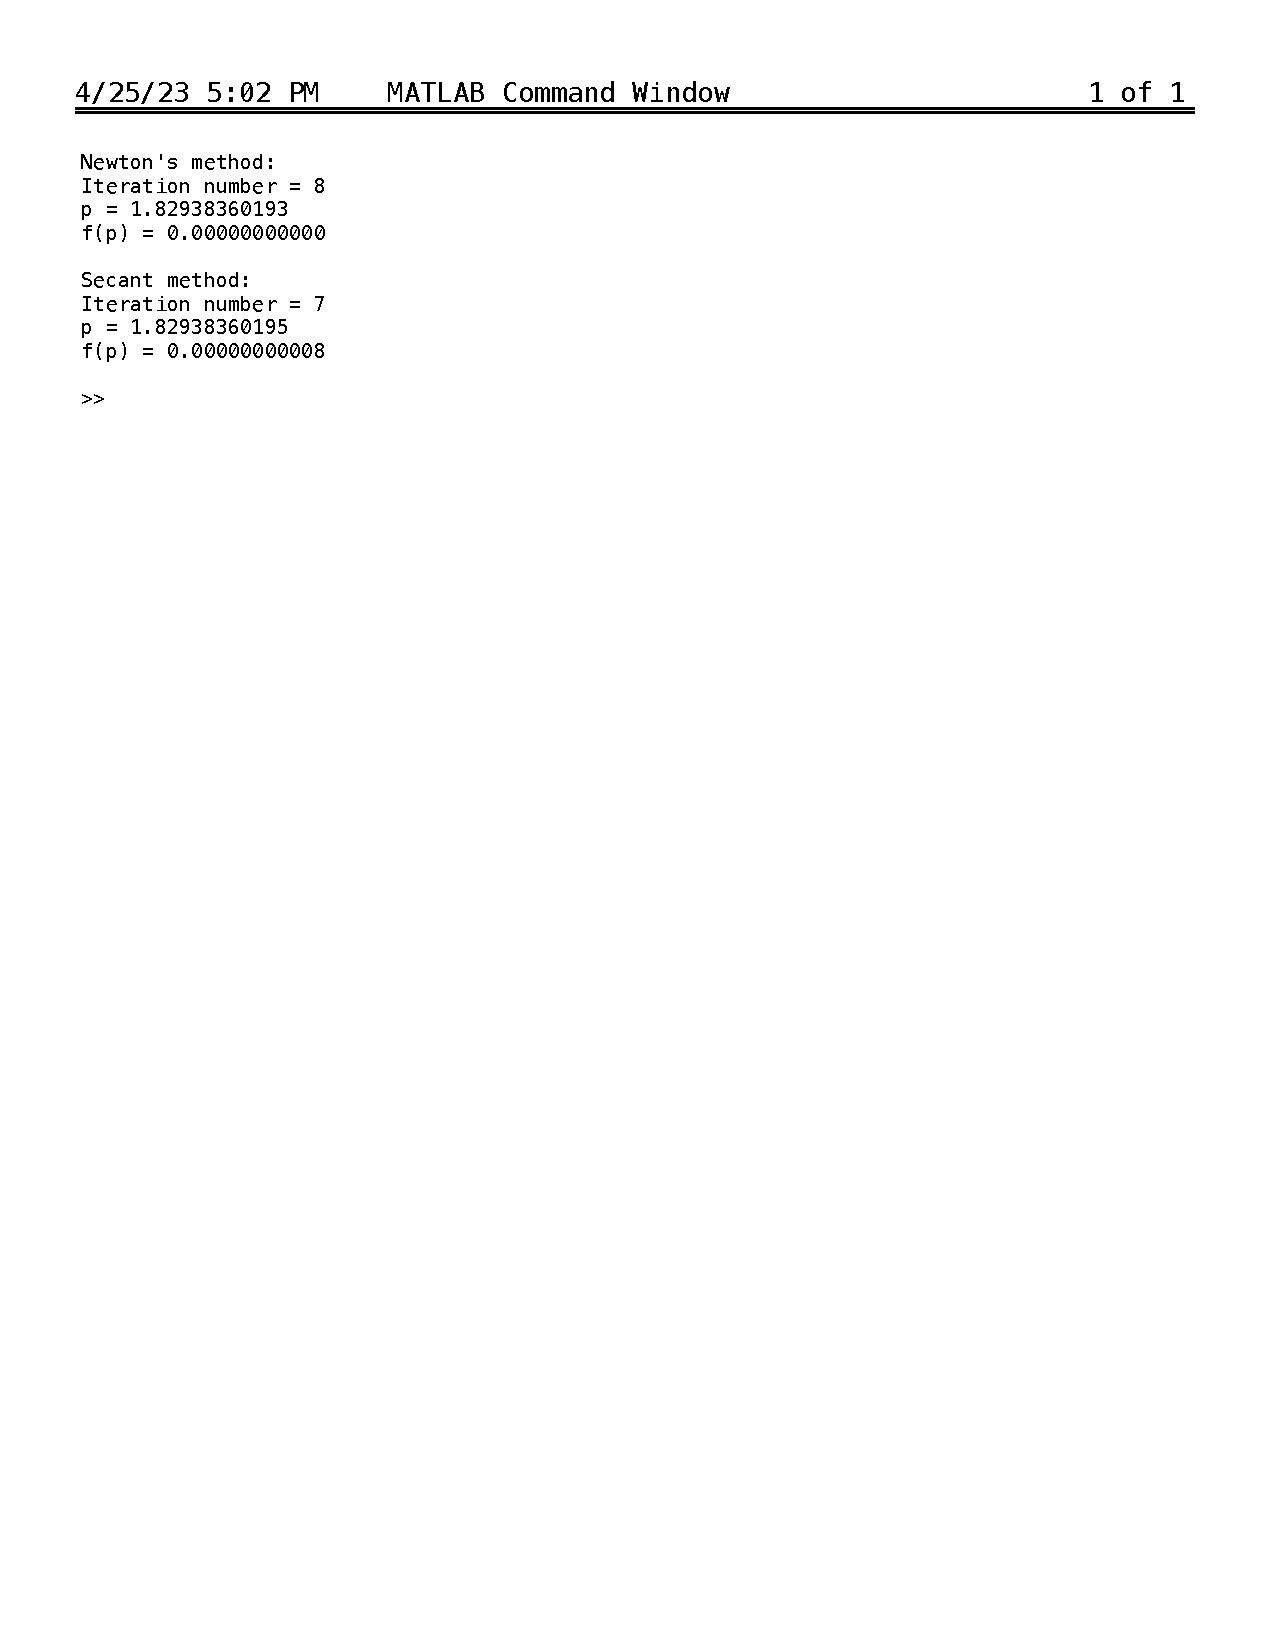
\includegraphics[width=\linewidth]{Command_hw_3_q_1_new.pdf} 
  \end{subfigure}% 
\end{figure}
\newpage
 %%%%%%%%%%%%%%%%%%%%%%%%%%%%%%

 \item \textbf{(C) Newton's Method for Optimization }\\
 Use Newton's method to approximate the value of $x$ that produces the point on the graph of $y = x^2$ that is closest to $(1, 0)$. Use the stopping criterion $|p_{n+1}-p_{n}|\leq 10^{-8}$ and the value $p_0 =1$. Report the approximation and the number of iterations needed to reach your computed solution. 

\textit{Hint: Minimize $d(x)^2$, where $d(x)$ represents the distance from $(x, x^2)$ to $(1, 0)$.}




\vspace{1em}
\textbf{Solution:}\par

$d(x)=\sqrt{x^4+(x-1)^2}$. Because distance is always non-negative and $x^2$ is monotone, $d(x)$ is minimized when $d(x)^2$ is minimized.\\ 
$(d(x)^2)'\in C^2[0,1]$. By observing the graph of $(d(x)^2)'$ there exists $p\in(0,1)$ s.t $(d(p)^2)'=0$ and $(d(p))''>0$, so there exists a sequence $(p_n)^{\infty}_{n=1}$ that converges to $p$ for any initial $p_0$ within some $\delta$ of $p$.\par
Let $f(x)=x-\frac{d'(x)^2}{d''(x)^2}=x-\frac{4x^3+2x-2}{12x^2+2}$ with initial estimate $p_0=1$.\\
It takes $6$ iterations to obtain a $10^{-8}$-accurate approximation with $p_6=0.58975451230$.
\begin{figure}[H]
  \centering
      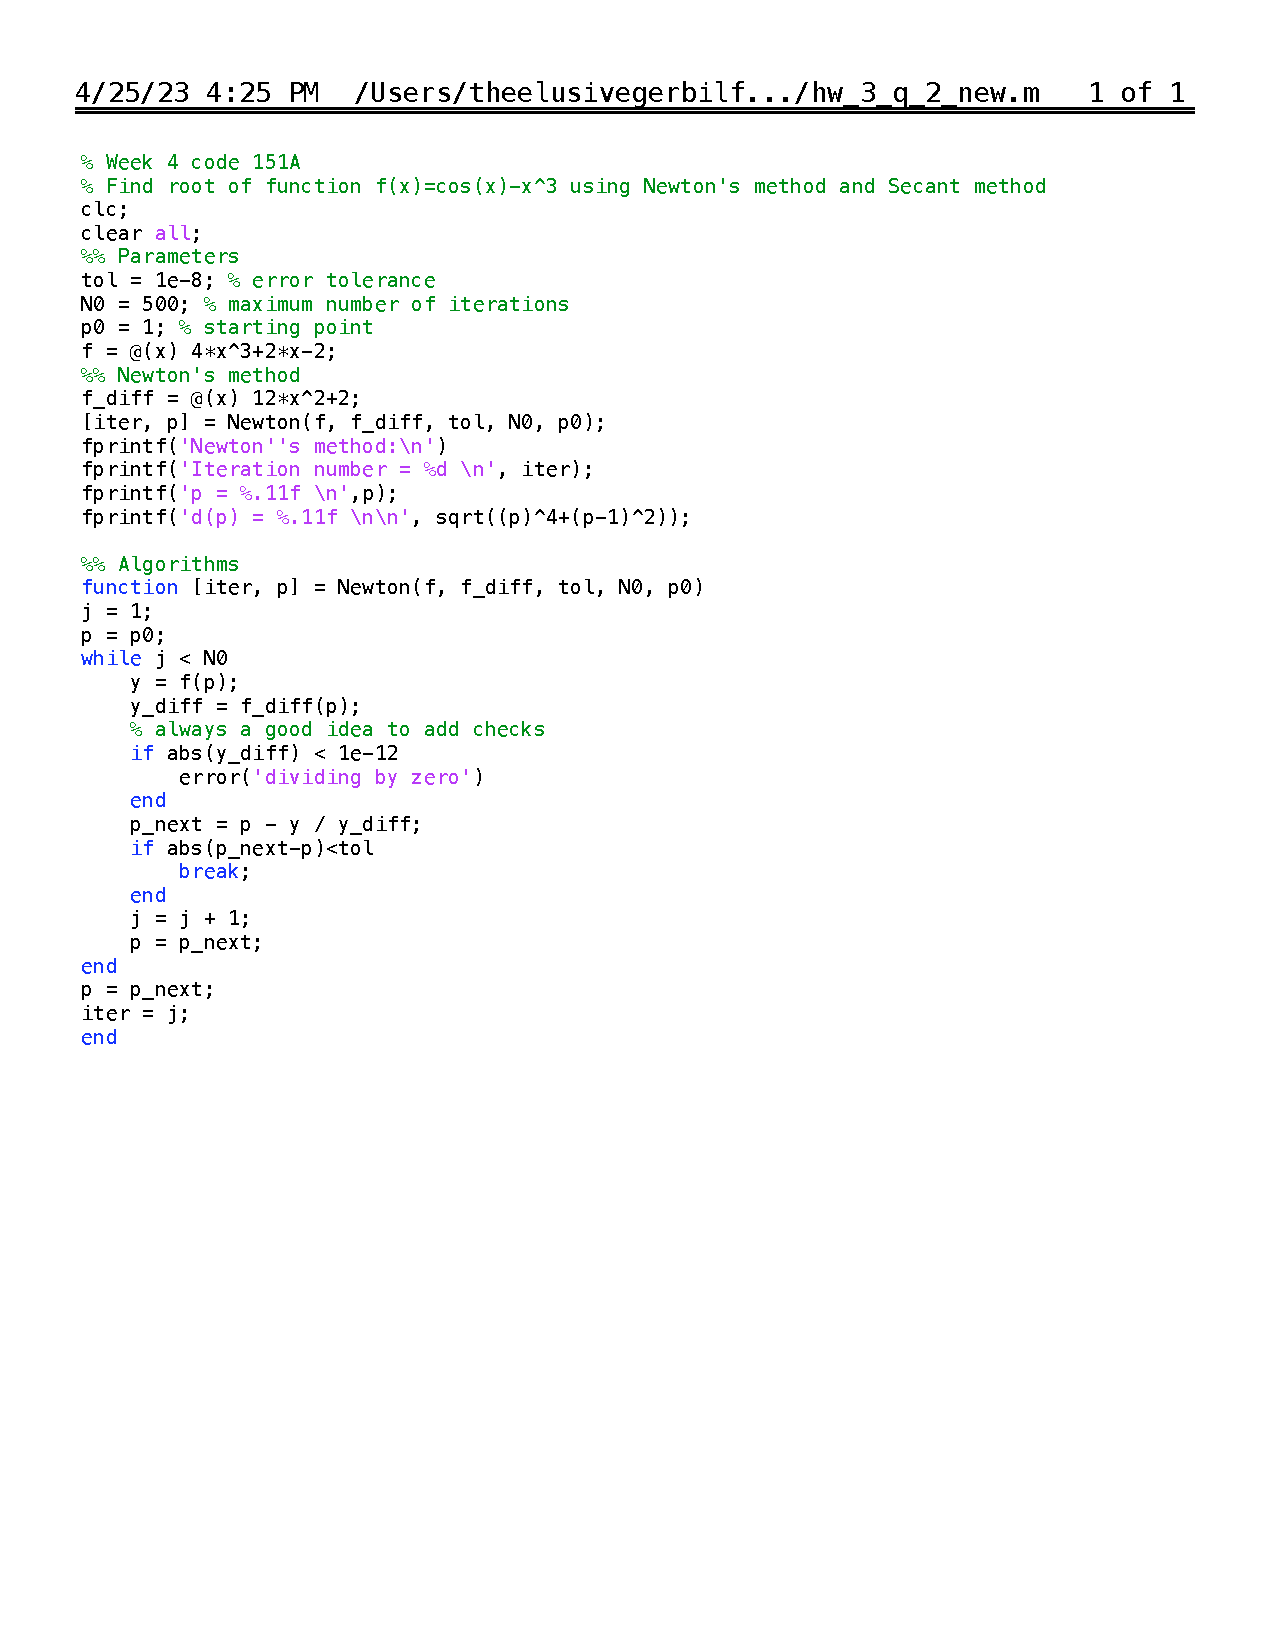
\includegraphics[trim=2cm 10cm 0 2cm, width=10cm]{hw_3_q_2_new.pdf}
      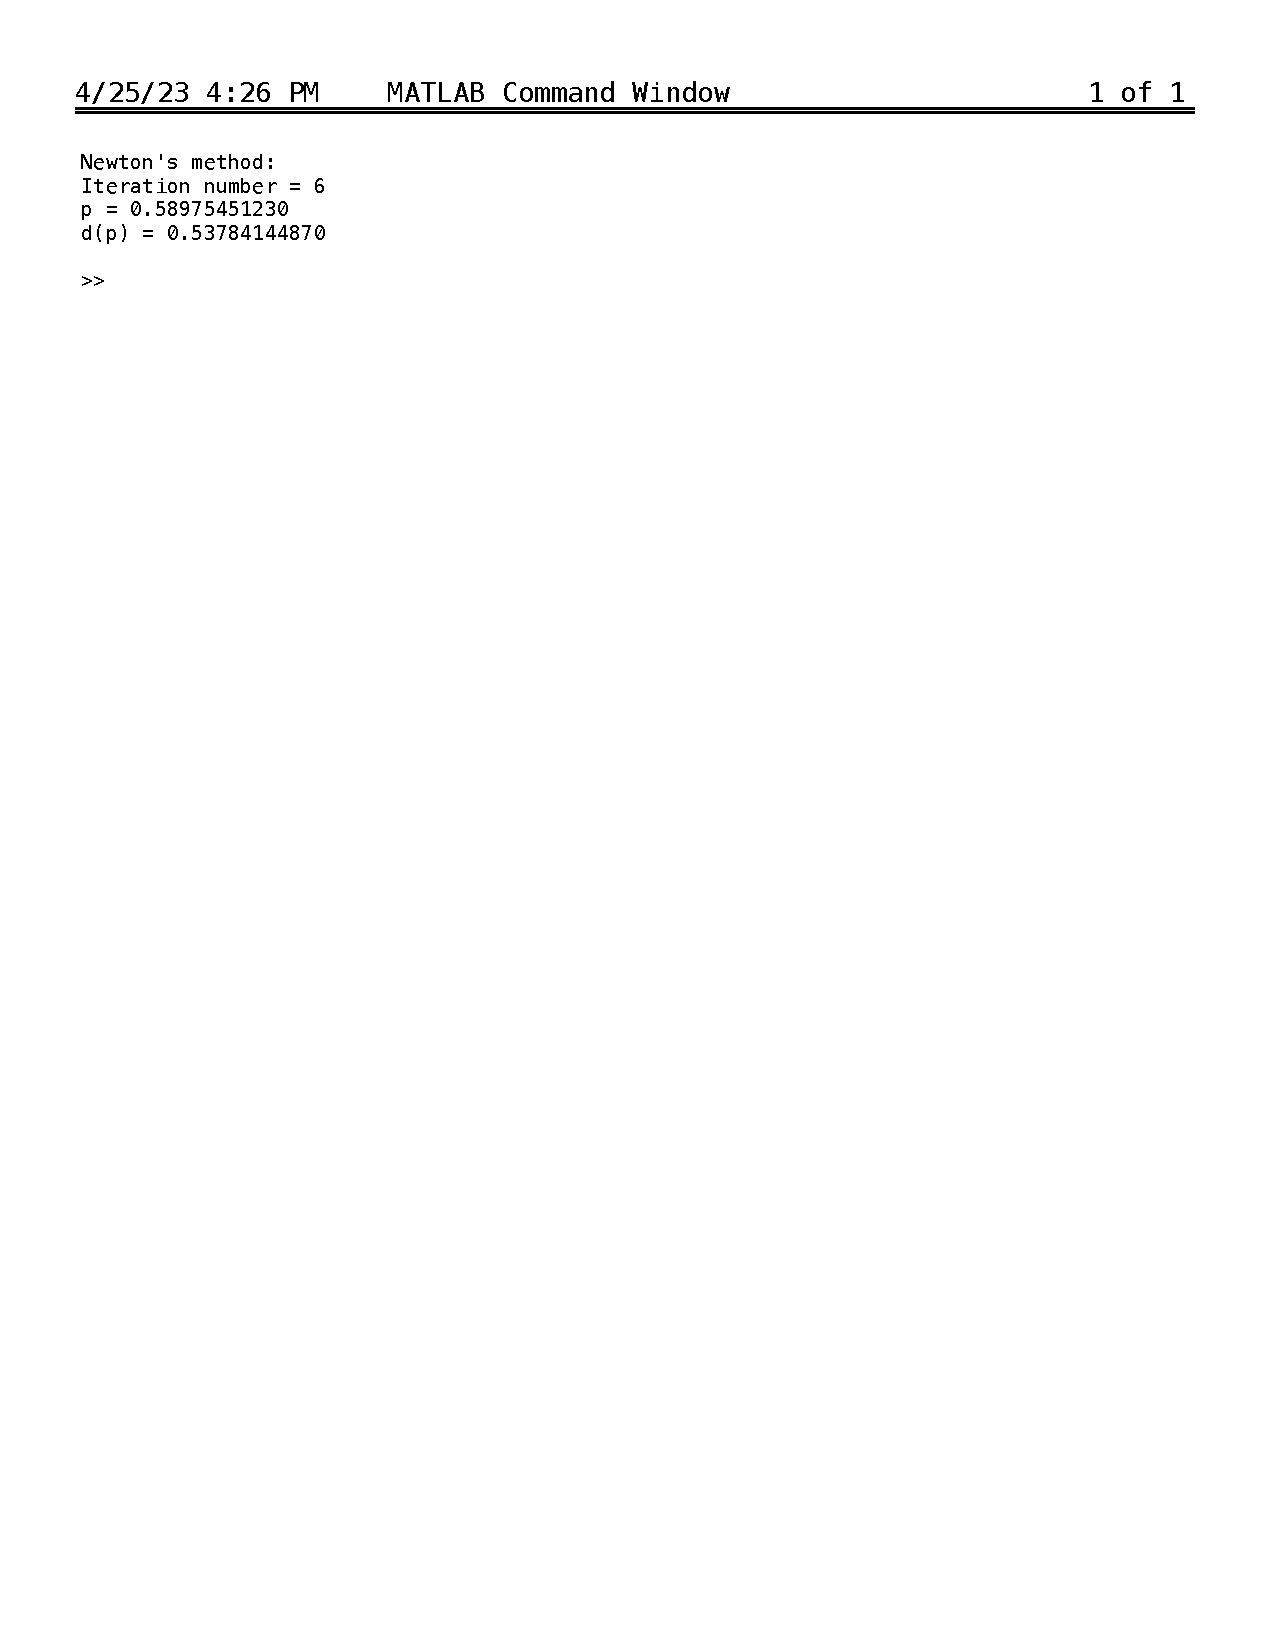
\includegraphics[trim=2cm 20cm 0 1cm, width=10cm]{Command_hw_3_q_2_new.pdf}
\end{figure}

\newpage

%%%%%%%%%%%%%%%%%%%%%%%%%%%%%%
\item \textbf{(T) Convergence Rate}
\begin{itemize} 
 
 
\item[a)] Show that the sequence $p_n=10^{-2^n}$ converges quadratically to zero.



 
\item[b)] Show that for any positive $k>1$, the sequence $p_n=10^{-n^k}$ does not converge quadratically to zero.


  
\item[c)] The sequence $p_n=\sqrt{p_{n-1}}$ starting at $p_0=1.5$ converges to $p=1$. Show that it is linearly convergent (without explicitly solving $p_n$ as a function of $n$).



 
 \item[d)] The sequence $p_n=p_{n-1}-\frac{1}{5} \, p_{n-1}^5$ starting at $p_0=0.5$ converges to $p=0$. Show that it converges sublinearly (without explicitly solving $p_n$ as a function of $n$).


 

\item[e)] Recall that a sequence $\{p_n\}$ converges \textit{superlinearly} to $p$ if 
\begin{align*}
\lim_{n\rightarrow \infty} \frac{|p_{n+1}-p|}{|p_{n}-p|} = 0.
\end{align*}
Show that if $p_n \rightarrow p$ of order $a$ for $a>1$, then $p_n$ converges superlinearly to $p$.



  
\end{itemize}
\vspace{1em}
\textbf{Solution:}\par 
\begin{itemize} 

  \item[a)]If $p_n$ converges to $p$ quadratically, it automatically has to converge linearly as well.$\displaystyle{\lim_{n\rightarrow\infty}}\frac{|p_{n+1}-0|}{|p_n-0|^2}
  =\displaystyle{\lim_{n\rightarrow\infty}}\frac{|10^{-2^{n+1}}-0|}{|10^{-2^n}-0|^2}
  =\displaystyle{\lim_{n\rightarrow\infty}}\frac{|10^{-2^{n+1}}|}{|10^{-2\cdot2^n}|}
  =\displaystyle{\lim_{n\rightarrow\infty}}\frac{|10^{-2^{n+1}}|}{|10^{-2^{n+1}}|}=1$\par 
  Therefore, by the definition of order of convergence, $p_n$ converges to $0$ with order of convergence $2$ and error constant $1$. Since the order is $2$, $p_n$ converges quadtratically to $0$.
   
  \item[b)] $\displaystyle{\lim_{n\rightarrow\infty}}\frac{|p_{n+1}-0|}{|p_n-0|^2}
  =\displaystyle{\lim_{n\rightarrow\infty}}\frac{|10^{-(n+1)^k}-0|}{|10^{-n^k}-0|^2}
  =\displaystyle{\lim_{n\rightarrow\infty}}\frac{|10^{-(n+1)^k}|}{|10^{-2\cdot n^k}|}
  =\displaystyle{\lim_{n\rightarrow\infty}}|10^{2\cdot n^k-(n+1)^k}|
  =\displaystyle{\lim_{n\rightarrow\infty}}|10^{(n+1)^k(2(\frac{n}{n+1})^k-1)}|
  =\infty$ because $(n+1)^k$ diverges to infinity while $2(\frac{n}{n+1})^k-1)$ converges to one, so $(n+1)^k(2(\frac{n}{n+1})^k-1)$ diverges to infinity$\Rightarrow |10^{(n+1)^k(2(\frac{n}{n+1})^k-1)}|$ diverges to infinity.
    
  \item[c)] $\displaystyle{\lim_{n\rightarrow\infty}}\frac{|p_{n+1}-1|}{|p_n-1|}
  =\displaystyle{\lim_{n\rightarrow\infty}}\frac{|\sqrt{p_n}-1|}{|p_n-1|}
  =\displaystyle{\lim_{n\rightarrow\infty}}\frac{1}{|\sqrt{p_n}+1|}=\frac{1}{2}$ because $p_n$ converges to 1.\par 
  Therefore, by the definition of order of convergence, $p_n$ converges to $1$ with order of convergence $1$ and error constant $\frac{1}{2}$. Since the order is $1$, $p_n$ converges linearly to $1$.
  
  \item[d)] $\displaystyle{\lim_{n\rightarrow\infty}}\frac{|p_{n+1}-0|}{|p_n-0|}
  =\displaystyle{\lim_{n\rightarrow\infty}}\frac{|p_n-\frac{1}{5}p_{n}^{5}|}{|p_n|}
  =\displaystyle{\lim_{n\rightarrow\infty}}|1-\frac{1}{5}p_{n}^{4}|=1$ because $p_n$ converges to 0.\par 
  Therefore, by the definition of order of convergence, $p_n$ converges to $0$ with order of convergence $1$ and error constant $1$. Since the order is $1$ and $\lambda\ge1$, $p_n$ converges sublinearly to $0$.
  
  \item[e)] If $\displaystyle{\lim_{n\rightarrow\infty}}\frac{|p_{n+1}-p|}{|p_n-p|^a}=\lambda\text{ for }\lambda\in\mathbb{R}^+$. 
  It follows $\displaystyle{\lim_{n\rightarrow\infty}}\frac{|p_{n+1}-p|}{|p_n-p|}=\lambda\displaystyle{\lim_{n\rightarrow\infty}}|p_n-p|^{a-1}$. 
  Because $p_n\rightarrow p$ and $a>1$, it follows that $\lambda\displaystyle{\lim_{n\rightarrow\infty}}|p_n-p|^{a-1}=0$.
  Therefore $\displaystyle{\lim_{n\rightarrow\infty}}\frac{|p_{n+1}-p|}{|p_n-p|}=0$. Hence $p_n\rightarrow p$ superlinearly whenever $p_n\rightarrow p$ of order $a>1$.
  
  \end{itemize}
\newpage
%%%%%%%%%%%%%%%%%%%%%%%%%%%%%%

\item \textbf{(T) Polynomial Approximation}\\
Let $f(x)=e^{2x}$ for $x\in[0,2]$. Find the Lagrange interpolating polynomial of degree-$2$, i.e. $P_2(x)$, using the nodes $x_0=0$, $x_1=1$, and $x_2=2$ and use it to approximate $f(1.5)$ i.e. $f(1.5)\approx P_2(1.5)$. 




\vspace{1em}
\textbf{Solution:}\par 
$P_2(x)=\frac{(x-1)(x-2)}{2}-e^2(x)(x-2)+\frac{e^4(x)(x-1)}{2}$\\
$P(1.5)=25.89110$, $f(1.5)=20.08554$ Error$=5.80556$
\newpage
%%%%%%%%%%%%%%%%%%%%%%%%%%%%%%%%%%%




\item \textbf{(T) Lagrange Interpolating Polynomials}\\
Consider the function $f(x)=\frac{14}{3}x^{100} -\frac{64}{59}x^{50}-97$. Find the Lagrange interpolating polynomial of degree-$200$ on $[-1,1]$ using equally spaced nodes $x_j = -1+j\, h$ for $j=0, \cdots, n$ with $h = \frac{1}{100}$.

\textit{Hint: The solution for this problem should only be one sentence, no computing or derivations are needed.}





\vspace{1em}
\textbf{Solution:}\par 
$P(x)=f(x)-\frac{f^{(n+1)}(\xi(x))}{(n+1)!}(x-x_0)(x-x_1)...(x-x_n)=f(x)=\frac{14}{3}x^{100} -\frac{64}{59}x^{50}-97$ because $f$ is only $101$ times differentiable.\par 
More clearly $P(x)=\frac{14}{3}x^{100} -\frac{64}{59}x^{50}-97$ over the interval.
\newpage
%%%%%%%%%%%%%%%%%%%%%%%%%%%%%%%%%%%






\item \textbf{(T) Lagrange Interpolating Polynomials}\\
Let $P_3(x)$ be the degree-$3$ Lagrange interpolating polynomial using the input-output pairs $(0,0)$, $(0.5,s)$, $(1,3)$, and $(2,2)$. Find the value of $s$ so that the coefficient of the cubic term $x^3$ in $P_3(x)$ is equal to $6$.

\vspace{1em}
\textbf{Solution:}\par 
$P_3(x)=f(x_0)L_0(x)+f(x_1)L_1(x)+f(x_2)L_2(x)+f(x_3)L_3(x)$\\
$f(0)=0\Rightarrow f(0)L_0(x)=0$\\
$f(0.5)L_1(x)=s\frac{x(x-1)(x-2)}{0.5\cdot(-0.5)\cdot(-1.5)}=\frac{8sx(x-1)(x-2)}{3}$\\
$f(1)L_2(x)=3\frac{x(x-0.5)(x-2)}{1\cdot0.5\cdot(-1)}=-6x(x-0.5)(x-2)$\\
$f(2)L_3(x)=2\frac{x(x-0.5)(x-1)}{2\cdot1.5\cdot1}=\frac{2x(x-0.5)(x-1)}{3}$\\
$f(x_0)L_0(x)+f(x_1)L_1(x)+f(x_2)L_2(x)+f(x_3)L_3(x)\\
=\frac{8sx(x-1)(x-2)}{3}-6x(x-0.5)(x-2)+\frac{2x(x-0.5)(x-1)}{3}\\
=\frac{8s-16}{3}x^3+(14-8s)x^2+\frac{16s-17}{3}x$\\
If $s=4.25$ then $P_3(x)=6x^3-20x^2+17x$



\end{enumerate}

\end{document}


